% PARTE 3: Ejercicios Propuestos y Soluciones Detalladas
% Guía de Cónicas - Grado 10

\section{Ejercicios Propuestos}

Ahora es tu turno de poner en práctica todo lo que has aprendido sobre las cónicas. Resuelve los siguientes ejercicios aplicando los conceptos de circunferencia, parábola, elipse, hipérbola y ecuación general de segundo grado. Las soluciones detalladas están en la siguiente sección, pero intenta resolverlos primero por tu cuenta.

\begin{ejercicio}{Circunferencia: Centro y Radio}
Una circunferencia tiene ecuación $x^2 + y^2 - 6x + 8y + 9 = 0$.
\begin{enumerate}[label=\alph*)]
    \item Encuentra el centro y el radio de la circunferencia
    \item Determina si el punto $P(1, -2)$ está dentro, sobre o fuera de la circunferencia
    \item Encuentra los puntos de intersección con el eje $x$
\end{enumerate}
\end{ejercicio}

\begin{ejercicio}{Circunferencia: Ecuación a partir de Condiciones}
Encuentra la ecuación de la circunferencia que:
\begin{enumerate}[label=\alph*)]
    \item Tiene centro en $C(2, -3)$ y pasa por el punto $P(5, 1)$
    \item Verifica si el punto $Q(-1, -7)$ pertenece a esta circunferencia
    \item Determina la longitud del diámetro
\end{enumerate}
\end{ejercicio}

\begin{ejercicio}{Parábola: Análisis Completo}
Dada la parábola con ecuación $y = -\frac{1}{4}x^2 + 2x + 3$:
\begin{enumerate}[label=\alph*)]
    \item Encuentra las coordenadas del vértice
    \item Determina el eje de simetría
    \item Encuentra las intersecciones con los ejes coordenados
    \item Determina si la parábola abre hacia arriba o hacia abajo
    \item Encuentra el valor máximo o mínimo de la función
\end{enumerate}
\end{ejercicio}

\begin{ejercicio}{Parábola: Aplicación con Trayectoria}
Un balón de fútbol es pateado desde el suelo y su trayectoria sigue la ecuación $h(x) = -0.05x^2 + 2x$, donde $h$ es la altura en metros y $x$ es la distancia horizontal en metros desde el punto de lanzamiento.
\begin{enumerate}[label=\alph*)]
    \item ¿Cuál es la altura máxima que alcanza el balón?
    \item ¿A qué distancia horizontal se encuentra cuando alcanza la altura máxima?
    \item ¿Cuál es el alcance total del lanzamiento (distancia donde el balón toca el suelo)?
    \item Si hay un arco de 2.5 metros de altura ubicado a 35 metros del punto de lanzamiento, ¿pasará el balón por encima del arco?
\end{enumerate}
\end{ejercicio}

\begin{ejercicio}{Elipse: Elementos y Gráfica}
Una elipse tiene ecuación $\frac{x^2}{25} + \frac{y^2}{9} = 1$.
\begin{enumerate}[label=\alph*)]
    \item Identifica el centro, los semiejes mayor y menor
    \item Encuentra las coordenadas de los focos
    \item Calcula la excentricidad
    \item Determina los vértices de la elipse
    \item Si un punto $P$ está sobre la elipse, verifica que la suma de sus distancias a los focos es constante
\end{enumerate}
\end{ejercicio}

\begin{ejercicio}{Hipérbola: Análisis y Propiedades}
Considera la hipérbola con ecuación $\frac{x^2}{16} - \frac{y^2}{9} = 1$.
\begin{enumerate}[label=\alph*)]
    \item Determina el centro y los vértices
    \item Encuentra las coordenadas de los focos
    \item Escribe las ecuaciones de las asíntotas
    \item Calcula la excentricidad
    \item Encuentra los puntos de la hipérbola cuando $x = 5$
\end{enumerate}
\end{ejercicio}

\begin{ejercicio}{Ecuación General: Identificación de Cónica}
Dada la ecuación $4x^2 + 9y^2 - 16x + 18y - 11 = 0$:
\begin{enumerate}[label=\alph*)]
    \item Identifica qué tipo de cónica representa
    \item Completa cuadrados para escribir la ecuación en forma estándar
    \item Encuentra el centro de la cónica
    \item Determina los elementos principales (semiejes, focos, etc.)
    \item Realiza un bosquejo de la gráfica indicando todos los elementos importantes
\end{enumerate}
\end{ejercicio}

\newpage

\section{Soluciones Detalladas}

\begin{solucion}[title=Solución Ejercicio 1: Circunferencia - Centro y Radio]
\textbf{Ecuación dada:} $x^2 + y^2 - 6x + 8y + 9 = 0$

\textbf{Parte a) Encontrar centro y radio}

\textbf{Paso 1:} Reorganizar términos por variable
\[
(x^2 - 6x) + (y^2 + 8y) + 9 = 0
\]

\textbf{Paso 2:} Completar cuadrados para $x$
\begin{align*}
x^2 - 6x &= (x - 3)^2 - 9
\end{align*}

\textbf{Paso 3:} Completar cuadrados para $y$
\begin{align*}
y^2 + 8y &= (y + 4)^2 - 16
\end{align*}

\textbf{Paso 4:} Sustituir en la ecuación original
\begin{align*}
(x - 3)^2 - 9 + (y + 4)^2 - 16 + 9 &= 0\\
(x - 3)^2 + (y + 4)^2 - 16 &= 0\\
(x - 3)^2 + (y + 4)^2 &= 16
\end{align*}

\textbf{Paso 5:} Identificar centro y radio
\[
\text{Centro: } C(3, -4), \quad \text{Radio: } r = \sqrt{16} = 4
\]

\textbf{Parte b) Posición del punto $P(1, -2)$}

\textbf{Paso 1:} Calcular la distancia del punto al centro
\begin{align*}
d &= \sqrt{(1-3)^2 + (-2-(-4))^2}\\
&= \sqrt{(-2)^2 + (2)^2}\\
&= \sqrt{4 + 4} = \sqrt{8} = 2\sqrt{2} \approx 2.83
\end{align*}

\textbf{Paso 2:} Comparar con el radio
Como $d = 2\sqrt{2} < 4 = r$, el punto está \textbf{dentro} de la circunferencia.

\textbf{Parte c) Intersecciones con el eje $x$}

En el eje $x$, tenemos $y = 0$. Sustituimos en la ecuación estándar:
\begin{align*}
(x - 3)^2 + (0 + 4)^2 &= 16\\
(x - 3)^2 + 16 &= 16\\
(x - 3)^2 &= 0\\
x - 3 &= 0\\
x &= 3
\end{align*}

La circunferencia toca el eje $x$ en un único punto: $(3, 0)$

\textbf{Verificación:} El centro está en $(3, -4)$ con radio 4. La distancia del centro al eje $x$ es $|-4| = 4$, que es exactamente el radio, confirmando que la circunferencia es tangente al eje $x$.

\begin{center}
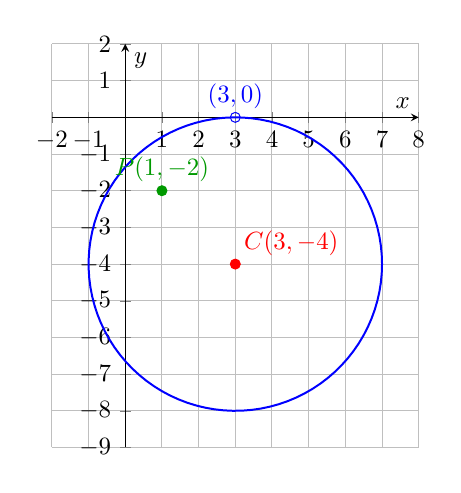
\begin{tikzpicture}[scale=0.9]
    \begin{axis}[
        axis lines=middle,
        xlabel=$x$,
        ylabel=$y$,
        xmin=-2, xmax=8,
        ymin=-9, ymax=2,
        grid=major,
        width=0.85\textwidth,
        height=0.6\textwidth,
        axis equal image,
        xtick={-2,-1,0,1,2,3,4,5,6,7,8},
        ytick={-9,-8,-7,-6,-5,-4,-3,-2,-1,0,1,2}
    ]
    % Circunferencia
    \addplot[blue, thick, domain=0:360, samples=100] ({3+4*cos(x)}, {-4+4*sin(x)});
    % Centro
    \addplot[mark=*, red] coordinates {(3,-4)} node[above right] {$C(3,-4)$};
    % Punto P
    \addplot[mark=*, green!60!black] coordinates {(1,-2)} node[above] {$P(1,-2)$};
    % Tangencia con eje x
    \addplot[mark=o, blue] coordinates {(3,0)} node[above] {$(3,0)$};
    \end{axis}
\end{tikzpicture}
\end{center}

\textbf{Respuesta:} \boxed{\text{a) Centro: } (3,-4), \text{ Radio: } 4; \text{ b) } P \text{ está dentro; c) Intersección: } (3,0)}
\end{solucion}

\begin{solucion}[title=Solución Ejercicio 2: Circunferencia - Ecuación a partir de Condiciones]
\textbf{Parte a) Ecuación con centro $C(2, -3)$ que pasa por $P(5, 1)$}

\textbf{Paso 1:} Calcular el radio usando la distancia de $C$ a $P$
\begin{align*}
r &= \sqrt{(5-2)^2 + (1-(-3))^2}\\
&= \sqrt{3^2 + 4^2}\\
&= \sqrt{9 + 16}\\
&= \sqrt{25} = 5
\end{align*}

\textbf{Paso 2:} Escribir la ecuación estándar
\[
(x - 2)^2 + (y + 3)^2 = 25
\]

\textbf{Paso 3:} Expandir para obtener la ecuación general
\begin{align*}
(x - 2)^2 + (y + 3)^2 &= 25\\
x^2 - 4x + 4 + y^2 + 6y + 9 &= 25\\
x^2 + y^2 - 4x + 6y + 13 &= 25\\
x^2 + y^2 - 4x + 6y - 12 &= 0
\end{align*}

\textbf{Parte b) Verificar si $Q(-1, -7)$ pertenece a la circunferencia}

\textbf{Método 1: Usando la ecuación estándar}
\begin{align*}
(-1 - 2)^2 + (-7 + 3)^2 &= (-3)^2 + (-4)^2\\
&= 9 + 16 = 25 \checkmark
\end{align*}

Como el resultado es igual a $r^2 = 25$, el punto $Q$ sí pertenece a la circunferencia.

\textbf{Método 2: Verificación con la ecuación general}
\begin{align*}
(-1)^2 + (-7)^2 - 4(-1) + 6(-7) - 12 &= 1 + 49 + 4 - 42 - 12\\
&= 0 \checkmark
\end{align*}

\textbf{Parte c) Longitud del diámetro}

El diámetro es el doble del radio:
\[
D = 2r = 2(5) = 10
\]

\begin{center}
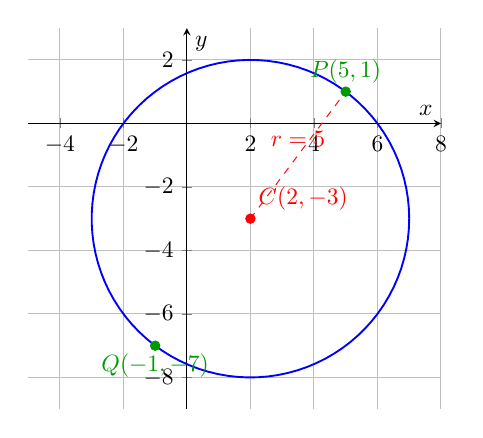
\begin{tikzpicture}[scale=0.85]
    \begin{axis}[
        axis lines=middle,
        xlabel=$x$,
        ylabel=$y$,
        xmin=-5, xmax=8,
        ymin=-9, ymax=3,
        grid=major,
        width=0.85\textwidth,
        height=0.6\textwidth,
        axis equal image
    ]
    % Circunferencia
    \addplot[blue, thick, domain=0:360, samples=100] ({2+5*cos(x)}, {-3+5*sin(x)});
    % Centro
    \addplot[mark=*, red] coordinates {(2,-3)} node[above right] {$C(2,-3)$};
    % Punto P
    \addplot[mark=*, green!60!black] coordinates {(5,1)} node[above] {$P(5,1)$};
    % Punto Q
    \addplot[mark=*, green!60!black] coordinates {(-1,-7)} node[below] {$Q(-1,-7)$};
    % Radio visualizado
    \draw[red, dashed] (axis cs:2,-3) -- (axis cs:5,1) node[midway, above] {$r=5$};
    \end{axis}
\end{tikzpicture}
\end{center}

\textbf{Respuesta:} \boxed{\text{a) } x^2 + y^2 - 4x + 6y - 12 = 0; \text{ b) } Q \text{ sí pertenece; c) Diámetro = 10}}
\end{solucion}

\begin{solucion}[title=Solución Ejercicio 3: Parábola - Análisis Completo]
\textbf{Ecuación:} $y = -\frac{1}{4}x^2 + 2x + 3$

\textbf{Parte a) Coordenadas del vértice}

Para una parábola $y = ax^2 + bx + c$, el vértice tiene coordenada $x = -\frac{b}{2a}$

\textbf{Paso 1:} Identificar coeficientes
\[
a = -\frac{1}{4}, \quad b = 2, \quad c = 3
\]

\textbf{Paso 2:} Calcular la coordenada $x$ del vértice
\[
x_v = -\frac{b}{2a} = -\frac{2}{2(-\frac{1}{4})} = -\frac{2}{-\frac{1}{2}} = 4
\]

\textbf{Paso 3:} Calcular la coordenada $y$ del vértice
\begin{align*}
y_v &= -\frac{1}{4}(4)^2 + 2(4) + 3\\
&= -\frac{1}{4}(16) + 8 + 3\\
&= -4 + 8 + 3 = 7
\end{align*}

Vértice: $V(4, 7)$

\textbf{Parte b) Eje de simetría}

El eje de simetría es la recta vertical $x = 4$

\textbf{Parte c) Intersecciones con los ejes}

\textbf{Intersección con el eje $y$:} Hacemos $x = 0$
\[
y = -\frac{1}{4}(0)^2 + 2(0) + 3 = 3
\]
Punto: $(0, 3)$

\textbf{Intersecciones con el eje $x$:} Hacemos $y = 0$
\begin{align*}
-\frac{1}{4}x^2 + 2x + 3 &= 0\\
\text{Multiplicamos por -4:} \quad x^2 - 8x - 12 &= 0
\end{align*}

Usando la fórmula cuadrática:
\begin{align*}
x &= \frac{8 \pm \sqrt{64 + 48}}{2} = \frac{8 \pm \sqrt{112}}{2}\\
&= \frac{8 \pm 4\sqrt{7}}{2} = 4 \pm 2\sqrt{7}
\end{align*}

\[
x_1 = 4 - 2\sqrt{7} \approx -1.29, \quad x_2 = 4 + 2\sqrt{7} \approx 9.29
\]

\textbf{Parte d) Dirección de apertura}

Como $a = -\frac{1}{4} < 0$, la parábola abre hacia abajo.

\textbf{Parte e) Valor máximo}

Como la parábola abre hacia abajo, tiene un máximo en el vértice: $y_{max} = 7$

\begin{center}
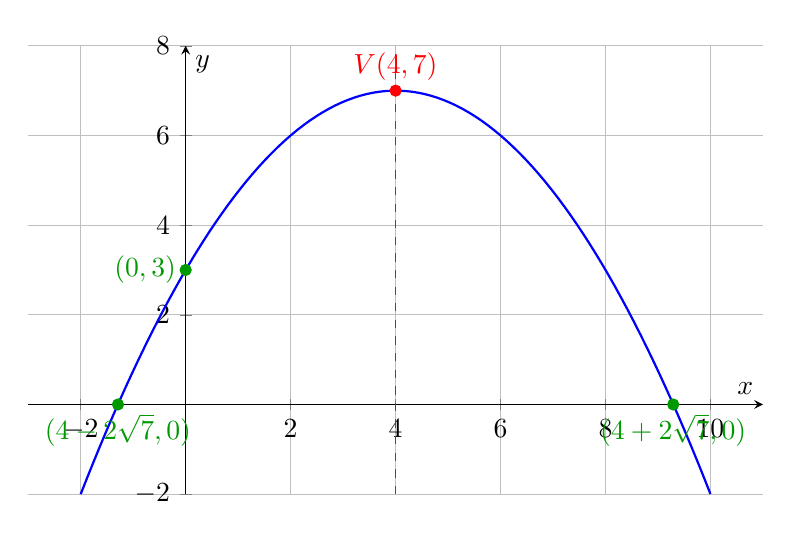
\begin{tikzpicture}[scale=1]
    \begin{axis}[
        axis lines=middle,
        xlabel=$x$,
        ylabel=$y$,
        xmin=-3, xmax=11,
        ymin=-2, ymax=8,
        grid=major,
        width=0.9\textwidth,
        height=0.6\textwidth
    ]
    % Parábola
    \addplot[blue, thick, domain=-2:10, samples=100] {-0.25*x^2 + 2*x + 3};
    % Vértice
    \addplot[mark=*, red] coordinates {(4,7)} node[above] {$V(4,7)$};
    % Intersección con eje y
    \addplot[mark=*, green!60!black] coordinates {(0,3)} node[left] {$(0,3)$};
    % Intersecciones con eje x
    \addplot[mark=*, green!60!black] coordinates {(-1.29,0)} node[below] {$(4-2\sqrt{7},0)$};
    \addplot[mark=*, green!60!black] coordinates {(9.29,0)} node[below] {$(4+2\sqrt{7},0)$};
    % Eje de simetría
    \draw[red, dashed] (axis cs:4,-2) -- (axis cs:4,8) node[above] {$x=4$};
    \end{axis}
\end{tikzpicture}
\end{center}

\textbf{Respuesta:} \boxed{\text{a) } V(4,7); \text{ b) } x=4; \text{ c) } (0,3), (4\pm2\sqrt{7},0); \text{ d) Abre hacia abajo; e) } y_{max}=7}
\end{solucion}

\begin{solucion}[title=Solución Ejercicio 4: Parábola - Aplicación con Trayectoria]
\textbf{Ecuación de trayectoria:} $h(x) = -0.05x^2 + 2x$

\textbf{Parte a) Altura máxima}

\textbf{Paso 1:} Identificar coeficientes
\[
a = -0.05, \quad b = 2, \quad c = 0
\]

\textbf{Paso 2:} Encontrar la coordenada $x$ del vértice
\[
x_v = -\frac{b}{2a} = -\frac{2}{2(-0.05)} = -\frac{2}{-0.1} = 20 \text{ metros}
\]

\textbf{Paso 3:} Calcular la altura máxima
\begin{align*}
h_{max} &= h(20) = -0.05(20)^2 + 2(20)\\
&= -0.05(400) + 40\\
&= -20 + 40 = 20 \text{ metros}
\end{align*}

\textbf{Parte b) Distancia horizontal en altura máxima}

Ya calculada: $x = 20$ metros

\textbf{Parte c) Alcance total}

El balón toca el suelo cuando $h(x) = 0$:
\begin{align*}
-0.05x^2 + 2x &= 0\\
x(-0.05x + 2) &= 0\\
x = 0 \text{ o } -0.05x + 2 &= 0\\
x = 0 \text{ o } x &= \frac{2}{0.05} = 40
\end{align*}

El alcance total es 40 metros.

\textbf{Parte d) ¿Pasa sobre el arco de 2.5 m a 35 m?}

\textbf{Paso 1:} Calcular la altura a 35 metros
\begin{align*}
h(35) &= -0.05(35)^2 + 2(35)\\
&= -0.05(1225) + 70\\
&= -61.25 + 70\\
&= 8.75 \text{ metros}
\end{align*}

\textbf{Paso 2:} Comparar con la altura del arco
Como $h(35) = 8.75 > 2.5$ metros, el balón sí pasa por encima del arco.

\begin{center}
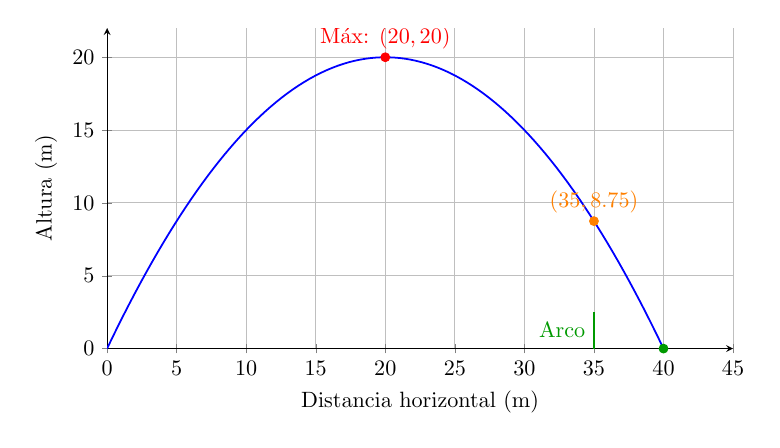
\begin{tikzpicture}[scale=0.8]
    \begin{axis}[
        axis lines=left,
        xlabel=Distancia horizontal (m),
        ylabel=Altura (m),
        xmin=0, xmax=45,
        ymin=0, ymax=22,
        grid=major,
        width=0.95\textwidth,
        height=0.55\textwidth
    ]
    % Trayectoria del balón
    \addplot[blue, thick, domain=0:40, samples=100] {-0.05*x^2 + 2*x};
    % Altura máxima
    \addplot[mark=*, red] coordinates {(20,20)} node[above] {Máx: $(20,20)$};
    % Arco
    \draw[green!60!black, very thick] (axis cs:35,0) -- (axis cs:35,2.5) node[midway, left] {Arco};
    % Punto sobre el arco
    \addplot[mark=*, orange] coordinates {(35,8.75)} node[above] {$(35, 8.75)$};
    % Alcance
    \addplot[mark=*, green!60!black] coordinates {(40,0)} node[below] {Alcance: 40 m};
    \end{axis}
\end{tikzpicture}
\end{center}

\textbf{Respuesta:} \boxed{\text{a) 20 m; b) 20 m; c) 40 m; d) Sí, pasa por encima (8.75 m > 2.5 m)}}
\end{solucion}

\begin{solucion}[title=Solución Ejercicio 5: Elipse - Elementos y Gráfica]
\textbf{Ecuación:} $\frac{x^2}{25} + \frac{y^2}{9} = 1$

\textbf{Parte a) Centro y semiejes}

\textbf{Paso 1:} Identificar la forma estándar $\frac{(x-h)^2}{a^2} + \frac{(y-k)^2}{b^2} = 1$
\[
\text{Centro: } (h,k) = (0,0)
\]

\textbf{Paso 2:} Identificar los semiejes
\[
a^2 = 25 \Rightarrow a = 5 \text{ (semieje mayor, horizontal)}
\]
\[
b^2 = 9 \Rightarrow b = 3 \text{ (semieje menor, vertical)}
\]

\textbf{Parte b) Coordenadas de los focos}

\textbf{Paso 1:} Calcular $c$ usando $c^2 = a^2 - b^2$
\begin{align*}
c^2 &= 25 - 9 = 16\\
c &= 4
\end{align*}

\textbf{Paso 2:} Como el eje mayor es horizontal, los focos están en:
\[
F_1(-4, 0) \text{ y } F_2(4, 0)
\]

\textbf{Parte c) Excentricidad}
\[
e = \frac{c}{a} = \frac{4}{5} = 0.8
\]

\textbf{Parte d) Vértices}

Vértices sobre el eje mayor: $V_1(-5, 0)$ y $V_2(5, 0)$

Vértices sobre el eje menor: $B_1(0, -3)$ y $B_2(0, 3)$

\textbf{Parte e) Verificación de la propiedad focal}

Para cualquier punto $P(x,y)$ sobre la elipse, la suma de distancias a los focos es:
\[
d(P,F_1) + d(P,F_2) = 2a = 10
\]

\textbf{Verificación con el punto $(3, \frac{12}{5})$:}

Primero verificamos que está en la elipse:
\[
\frac{3^2}{25} + \frac{(12/5)^2}{9} = \frac{9}{25} + \frac{144/25}{9} = \frac{9}{25} + \frac{16}{25} = 1 \checkmark
\]

Calculamos las distancias:
\begin{align*}
d(P,F_1) &= \sqrt{(3-(-4))^2 + (12/5-0)^2} = \sqrt{49 + 144/25} = \sqrt{1369/25} = 37/5\\
d(P,F_2) &= \sqrt{(3-4)^2 + (12/5-0)^2} = \sqrt{1 + 144/25} = \sqrt{169/25} = 13/5\\
\text{Suma: } &\frac{37}{5} + \frac{13}{5} = \frac{50}{5} = 10 = 2a \checkmark
\end{align*}

\begin{center}
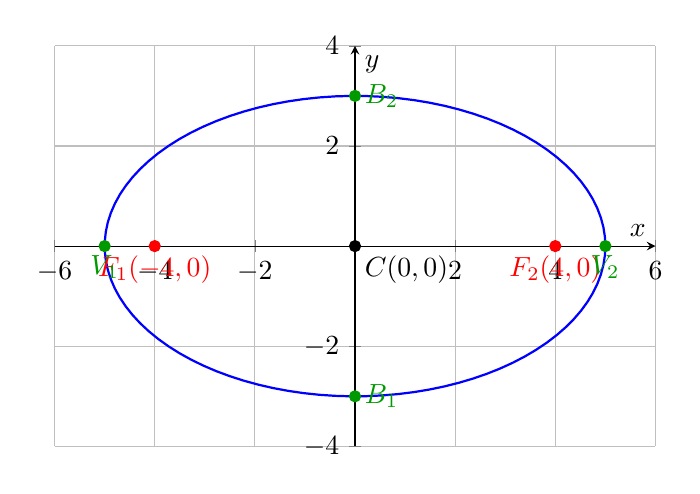
\begin{tikzpicture}[scale=1]
    \begin{axis}[
        axis lines=middle,
        xlabel=$x$,
        ylabel=$y$,
        xmin=-6, xmax=6,
        ymin=-4, ymax=4,
        grid=major,
        width=0.9\textwidth,
        height=0.55\textwidth,
        axis equal image
    ]
    % Elipse
    \addplot[blue, thick, domain=0:360, samples=100] ({5*cos(x)}, {3*sin(x)});
    % Centro
    \addplot[mark=*, black] coordinates {(0,0)} node[below right] {$C(0,0)$};
    % Focos
    \addplot[mark=*, red] coordinates {(-4,0)} node[below] {$F_1(-4,0)$};
    \addplot[mark=*, red] coordinates {(4,0)} node[below] {$F_2(4,0)$};
    % Vértices eje mayor
    \addplot[mark=*, green!60!black] coordinates {(-5,0)} node[below] {$V_1$};
    \addplot[mark=*, green!60!black] coordinates {(5,0)} node[below] {$V_2$};
    % Vértices eje menor
    \addplot[mark=*, green!60!black] coordinates {(0,-3)} node[right] {$B_1$};
    \addplot[mark=*, green!60!black] coordinates {(0,3)} node[right] {$B_2$};
    \end{axis}
\end{tikzpicture}
\end{center}

\textbf{Respuesta:} \boxed{\text{Centro: } (0,0), a=5, b=3; \text{ Focos: } (\pm4,0); e=0.8; \text{ Vértices: } (\pm5,0), (0,\pm3)}
\end{solucion}

\begin{solucion}[title=Solución Ejercicio 6: Hipérbola - Análisis y Propiedades]
\textbf{Ecuación:} $\frac{x^2}{16} - \frac{y^2}{9} = 1$

\textbf{Parte a) Centro y vértices}

\textbf{Paso 1:} Identificar la forma estándar $\frac{(x-h)^2}{a^2} - \frac{(y-k)^2}{b^2} = 1$
\[
\text{Centro: } (h,k) = (0,0)
\]

\textbf{Paso 2:} Identificar los parámetros
\[
a^2 = 16 \Rightarrow a = 4, \quad b^2 = 9 \Rightarrow b = 3
\]

\textbf{Paso 3:} Los vértices están sobre el eje transverso (horizontal):
\[
V_1(-4, 0) \text{ y } V_2(4, 0)
\]

\textbf{Parte b) Coordenadas de los focos}

\textbf{Paso 1:} Calcular $c$ usando $c^2 = a^2 + b^2$ (¡nota el signo + para hipérbolas!)
\begin{align*}
c^2 &= 16 + 9 = 25\\
c &= 5
\end{align*}

\textbf{Paso 2:} Los focos están en:
\[
F_1(-5, 0) \text{ y } F_2(5, 0)
\]

\textbf{Parte c) Ecuaciones de las asíntotas}

Para una hipérbola horizontal centrada en el origen:
\[
y = \pm\frac{b}{a}x = \pm\frac{3}{4}x
\]

Las asíntotas son: $y = \frac{3}{4}x$ y $y = -\frac{3}{4}x$

\textbf{Parte d) Excentricidad}
\[
e = \frac{c}{a} = \frac{5}{4} = 1.25
\]

Nota: En hipérbolas, siempre $e > 1$.

\textbf{Parte e) Puntos cuando $x = 5$}

Sustituimos $x = 5$ en la ecuación:
\begin{align*}
\frac{25}{16} - \frac{y^2}{9} &= 1\\
\frac{y^2}{9} &= \frac{25}{16} - 1 = \frac{25-16}{16} = \frac{9}{16}\\
y^2 &= 9 \cdot \frac{9}{16} = \frac{81}{16}\\
y &= \pm\frac{9}{4}
\end{align*}

Los puntos son: $(5, \frac{9}{4})$ y $(5, -\frac{9}{4})$

\begin{center}
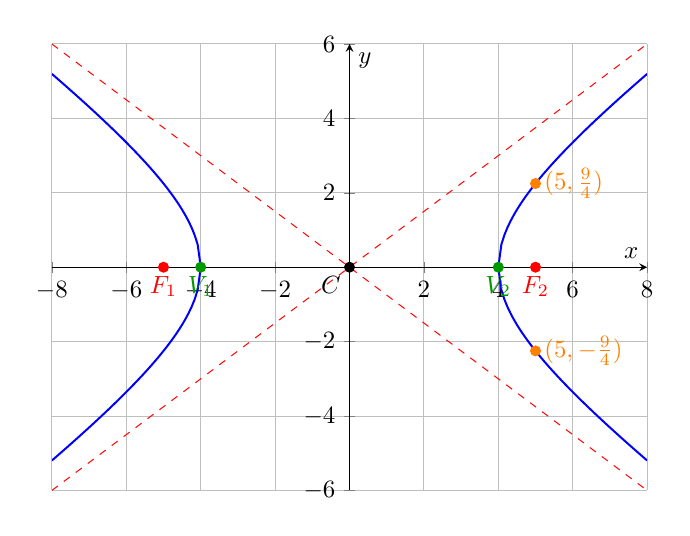
\begin{tikzpicture}[scale=0.9]
    \begin{axis}[
        axis lines=middle,
        xlabel=$x$,
        ylabel=$y$,
        xmin=-8, xmax=8,
        ymin=-6, ymax=6,
        grid=major,
        width=0.9\textwidth,
        height=0.65\textwidth,
        axis equal image
    ]
    % Hipérbola rama derecha
    \addplot[blue, thick, domain=4:8, samples=50] {3*sqrt(x^2/16 - 1)};
    \addplot[blue, thick, domain=4:8, samples=50] {-3*sqrt(x^2/16 - 1)};
    % Hipérbola rama izquierda
    \addplot[blue, thick, domain=-8:-4, samples=50] {3*sqrt(x^2/16 - 1)};
    \addplot[blue, thick, domain=-8:-4, samples=50] {-3*sqrt(x^2/16 - 1)};
    % Asíntotas
    \addplot[red, dashed, domain=-8:8] {0.75*x};
    \addplot[red, dashed, domain=-8:8] {-0.75*x};
    % Centro
    \addplot[mark=*, black] coordinates {(0,0)} node[below left] {$C$};
    % Vértices
    \addplot[mark=*, green!60!black] coordinates {(-4,0)} node[below] {$V_1$};
    \addplot[mark=*, green!60!black] coordinates {(4,0)} node[below] {$V_2$};
    % Focos
    \addplot[mark=*, red] coordinates {(-5,0)} node[below] {$F_1$};
    \addplot[mark=*, red] coordinates {(5,0)} node[below] {$F_2$};
    % Puntos en x=5
    \addplot[mark=*, orange] coordinates {(5,2.25)} node[right] {$(5,\frac{9}{4})$};
    \addplot[mark=*, orange] coordinates {(5,-2.25)} node[right] {$(5,-\frac{9}{4})$};
    \end{axis}
\end{tikzpicture}
\end{center}

\textbf{Respuesta:} \boxed{\text{Centro: } (0,0), V(\pm4,0); \text{ Focos: } (\pm5,0); \text{ Asíntotas: } y=\pm\frac{3}{4}x; e=1.25}
\end{solucion}

\begin{solucion}[title=Solución Ejercicio 7: Ecuación General - Identificación de Cónica]
\textbf{Ecuación:} $4x^2 + 9y^2 - 16x + 18y - 11 = 0$

\textbf{Parte a) Identificar el tipo de cónica}

Observamos los coeficientes de $x^2$ y $y^2$:
- Coeficiente de $x^2$: 4 (positivo)
- Coeficiente de $y^2$: 9 (positivo)
- Ambos coeficientes son positivos y diferentes

Por lo tanto, es una \textbf{elipse}.

\textbf{Parte b) Completar cuadrados}

\textbf{Paso 1:} Agrupar términos
\[
4x^2 - 16x + 9y^2 + 18y = 11
\]

\textbf{Paso 2:} Factorizar los coeficientes principales
\[
4(x^2 - 4x) + 9(y^2 + 2y) = 11
\]

\textbf{Paso 3:} Completar cuadrados dentro de cada paréntesis

Para $x$: $x^2 - 4x = (x-2)^2 - 4$

Para $y$: $y^2 + 2y = (y+1)^2 - 1$

\textbf{Paso 4:} Sustituir
\begin{align*}
4[(x-2)^2 - 4] + 9[(y+1)^2 - 1] &= 11\\
4(x-2)^2 - 16 + 9(y+1)^2 - 9 &= 11\\
4(x-2)^2 + 9(y+1)^2 &= 11 + 16 + 9\\
4(x-2)^2 + 9(y+1)^2 &= 36
\end{align*}

\textbf{Paso 5:} Dividir entre 36 para forma estándar
\[
\frac{(x-2)^2}{9} + \frac{(y+1)^2}{4} = 1
\]

\textbf{Parte c) Centro de la elipse}
\[
\text{Centro: } (h,k) = (2,-1)
\]

\textbf{Parte d) Elementos principales}

\textbf{Semiejes:}
\[
a^2 = 9 \Rightarrow a = 3 \text{ (semieje mayor, horizontal)}
\]
\[
b^2 = 4 \Rightarrow b = 2 \text{ (semieje menor, vertical)}
\]

\textbf{Distancia focal:}
\begin{align*}
c^2 &= a^2 - b^2 = 9 - 4 = 5\\
c &= \sqrt{5}
\end{align*}

\textbf{Focos:}
\[
F_1(2-\sqrt{5}, -1) \text{ y } F_2(2+\sqrt{5}, -1)
\]

\textbf{Vértices sobre eje mayor:}
\[
V_1(-1, -1) \text{ y } V_2(5, -1)
\]

\textbf{Vértices sobre eje menor:}
\[
B_1(2, -3) \text{ y } B_2(2, 1)
\]

\textbf{Excentricidad:}
\[
e = \frac{c}{a} = \frac{\sqrt{5}}{3} \approx 0.745
\]

\textbf{Parte e) Bosquejo de la gráfica}

\begin{center}
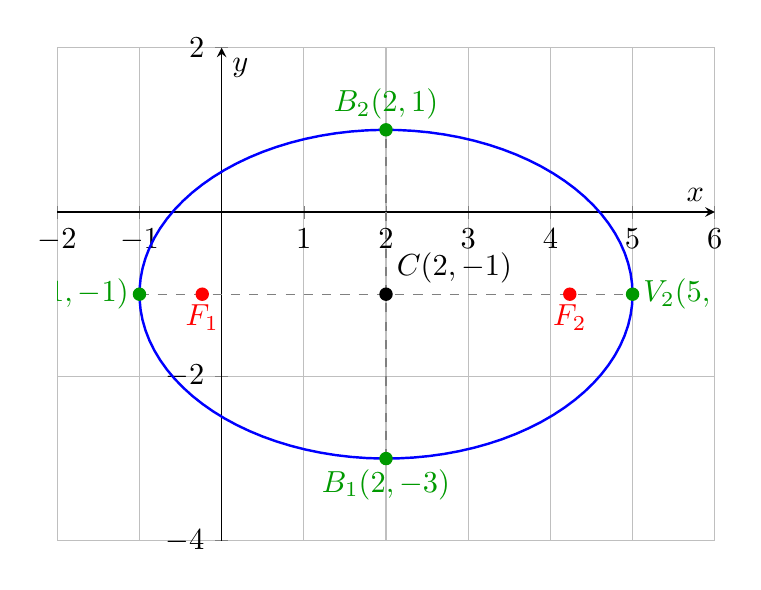
\begin{tikzpicture}[scale=1.1]
    \begin{axis}[
        axis lines=middle,
        xlabel=$x$,
        ylabel=$y$,
        xmin=-2, xmax=6,
        ymin=-4, ymax=2,
        grid=major,
        width=0.9\textwidth,
        height=0.6\textwidth,
        axis equal image
    ]
    % Elipse
    \addplot[blue, thick, domain=0:360, samples=100] ({2+3*cos(x)}, {-1+2*sin(x)});
    % Centro
    \addplot[mark=*, black] coordinates {(2,-1)} node[above right] {$C(2,-1)$};
    % Focos
    \addplot[mark=*, red] coordinates {(2-2.236,-1)} node[below] {$F_1$};
    \addplot[mark=*, red] coordinates {(2+2.236,-1)} node[below] {$F_2$};
    % Vértices eje mayor
    \addplot[mark=*, green!60!black] coordinates {(-1,-1)} node[left] {$V_1(-1,-1)$};
    \addplot[mark=*, green!60!black] coordinates {(5,-1)} node[right] {$V_2(5,-1)$};
    % Vértices eje menor
    \addplot[mark=*, green!60!black] coordinates {(2,-3)} node[below] {$B_1(2,-3)$};
    \addplot[mark=*, green!60!black] coordinates {(2,1)} node[above] {$B_2(2,1)$};
    % Ejes de la elipse
    \draw[gray, dashed] (axis cs:-1,-1) -- (axis cs:5,-1);
    \draw[gray, dashed] (axis cs:2,-3) -- (axis cs:2,1);
    \end{axis}
\end{tikzpicture}
\end{center}

\textbf{Respuesta:} \boxed{\text{Elipse: } \frac{(x-2)^2}{9} + \frac{(y+1)^2}{4} = 1; \text{ Centro: } (2,-1); a=3, b=2, c=\sqrt{5}}
\end{solucion}